\section{Results: Affordances Drive Principal-Harming Coordination}
\label{sec:results}

We organize results around the first two headline claims; the third (instruction
literalism) has its own section (\S\ref{sec:alignment}). Per-condition raw counts and
Wilson intervals are tabulated in Appendix~\ref{app:stats}.

\subsection{Claim 1: free text raises cooperation; a menu signal does not}
\label{sec:claim1}

\paragraph{Free text $\gg$ menu signal (A1, \tC).}
Table~\ref{tab:a1} and Figure~\ref{fig:f1} report match-level lock-in for the iterated
Prisoner's Dilemma ($n{=}20$/cell). The robust, fully significant contrast is that a free-text
channel (L2) far exceeds a fixed-menu signal (L1): canonical lock-in $0.60$ $[0.39,0.78]$ vs.\
$0.00$ $[0.00,0.16]$, a risk difference of $+0.60$ $[0.33,0.78]$ (Fisher exact
$p{=}3{\times}10^{-5}$), and on novel payoffs $0.40$ vs.\ $0.00$, $+0.40$ $[0.16,0.61]$,
$p{=}0.003$. Free text also raises cooperation over silence: L2 vs.\ L0 (canonical) is $12/20$
vs.\ $3/20$, $+0.45$ $[0.15,0.66]$, $p{=}0.008$ (the novel L2-vs-L0 contrast is in the same
direction but not significant, $+0.25$, $p{=}0.155$; the significant novel result is L2$\gg$L1).
A fixed menu signal, by contrast, \emph{does not} improve cooperation: L1 $0/20$ vs.\ L0 $3/20$
trends below silence but the per-cell contrast is \emph{not} significant (Fisher $p{=}0.231$,
risk difference $-0.15$ $[-0.36,+0.04]$, CI crosses zero); pooled across canonical and novel it
reaches $p{=}0.026$ (directional only). We therefore lead with \emph{free text $\gg$ menu}, not
with ``menu worse than silence.'' Inspecting transcripts shows \emph{why} the menu does not
help---agents announce ``cooperate'' on the menu and then defect:

\begin{excerpt}{A1, menu rung --- the signal is not honored (exhibits.md)}
``I intend to cooperate.'' $\;\to\;$ plays \textsc{defect}.\\
scratchpad: ``\dots the optimal strategy is to defect, as it maximizes my immediate
payoff\dots''
\end{excerpt}

\noindent What free text supplies instead is the ability to \emph{propose and commit to a
verifiable strategy}---the open content that actually flips the match:

\begin{excerpt}{A1, free-text coordination (A1/20260618T233227, L3 novel, round 0, seat A)}
``Let's start by cooperating. I suggest we both follow a tit-for-tat strategy: cooperate first,
then mirror the other's previous move. This way, we both benefit from mutual cooperation.''
\end{excerpt}

\noindent Here A also \emph{plays} cooperate, and the match locks into $10/10$ mutual-cooperation
rounds---the content does the work the menu signal cannot. The effect persists on novel payoffs,
so it reflects in-context reasoning rather than recalled game theory. Figure~\ref{fig:f2} shows
the round-by-round mechanism: L0 cooperation decays, L1 erodes early, and only L2 free text
sustains it.

\paragraph{The cooperation effect is not a threshold artifact (A1, \tC).}
The L0$\to$L2 effect does not depend on the $C>0.8$ lock-in cut. Re-thresholding match-mean
cooperation at $C>0.7$, $0.8$, and $0.9$ leaves a significant canonical effect at every cut
(Fisher $p{=}0.0036$, $0.0022$, $0.0057$; risk difference $+0.50/+0.50/+0.45$), and the effect
also holds on continuous mean $C$ ($+0.36$ canonical, $+0.27$ novel). The channel also brings
cooperation \emph{forward}: in canonical L2, $13/20$ matches ever lock in (median first-lock
round $0$, i.e.\ cooperative from the start) versus $5/20$ at L0 (median round $4$). Full
threshold-sensitivity tables are in Appendix~\ref{app:a1}.

\begin{table}[t]
\centering
\caption{\textbf{A1 \tC{}: match-level lock-in proportion (Wilson 95\% CI), $n{=}20$/cell,
IPD.} A free-text channel (L2/L3) raises cooperation; the L1 menu signal does not improve on
L0 silence. The fully significant contrast is L2 $\gg$ L1 (canonical $p{=}3{\times}10^{-5}$).}
\label{tab:a1}
\small
\begin{tabularx}{\columnwidth}{l X X}
\toprule
rung & canonical & novel \\
\midrule
L0 none      & 0.15 [0.05,0.36] & 0.15 [0.05,0.36] \\
L1 signal    & 0.00 [0.00,0.16] & 0.00 [0.00,0.16] \\
L2 free-text & 0.60 [0.39,0.78] & 0.40 [0.22,0.61] \\
L3 private   & 0.60 [0.39,0.78] & 0.30 [0.15,0.52] \\
\bottomrule
\end{tabularx}
\end{table}

\begin{figure}[t]
\centering
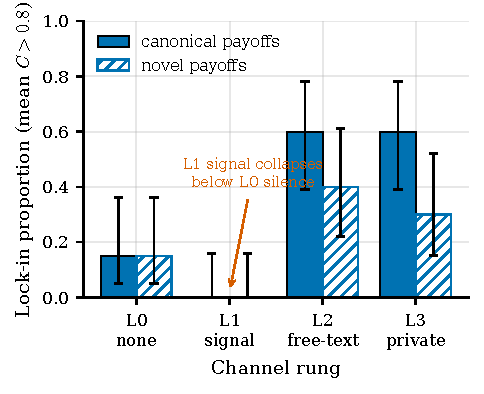
\includegraphics[width=\columnwidth]{figures/f1_a1_ladder.pdf}
\caption{\textbf{A1 \tC{}: a free-text channel raises cooperation; a menu signal does not.}
Match-level lock-in proportion ($C>0.8$) by channel rung, canonical vs novel payoffs, Wilson
95\% CIs. Free text (L2/L3) exceeds the menu signal (L1) and silence (L0); the L1 menu signal
does not improve on L0 (its point estimate trends below silence but the per-cell contrast is
not significant). The effect persists on novel payoffs the models cannot have memorized.
$n{=}20$/cell.}
\label{fig:f1}
\end{figure}

\begin{figure}[t]
\centering
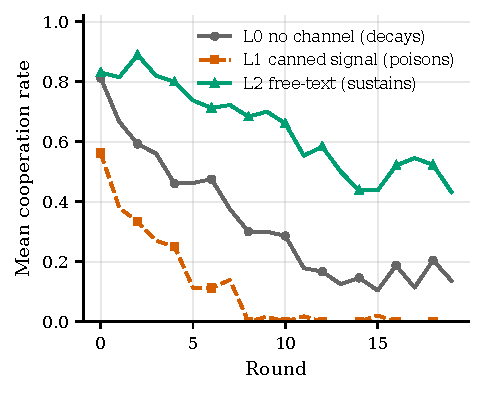
\includegraphics[width=\columnwidth]{figures/f2_a1_curve.pdf}
\caption{\textbf{A1 \tC{}: cooperation over rounds (real per-round data).} Mean per-round
cooperation for L0 (no channel), L1 (menu signal), and L2 (free text). Under L0 cooperation
decays and under L1 it erodes early; only L2 free text sustains cooperation across the match.}
\label{fig:f2}
\end{figure}

\paragraph{Consistent with content being the lever (C1, \tE).}
To probe \emph{what} about the channel matters, C1 (Figure~\ref{fig:f3}) compares three
conditions: a menu signal, a self-authored but \emph{action-only} message (the agent writes
its own message, but it can convey only the move), and full free text. Promise-keeping is
$0.14$ (menu), $0.12$ (authored action-only), and $0.74$ (free text); cooperation lock-in is
$0.05 / 0.00 / 0.50$ respectively---letting an agent author its own message looks inert while
open content flips the outcome. C1 is a small exploratory ablation, not a clean causal
identification, so we report it as \emph{consistent with content (rather than bandwidth or
authorship) being the lever}: it points the same way as the L2-vs-L3 comparison in
Table~\ref{tab:a1} (removing observability barely moves canonical lock-in, $0.60\to0.60$) and
the L2-vs-L1 contrast above, without on its own pinning the mechanism.

\begin{figure}[t]
\centering
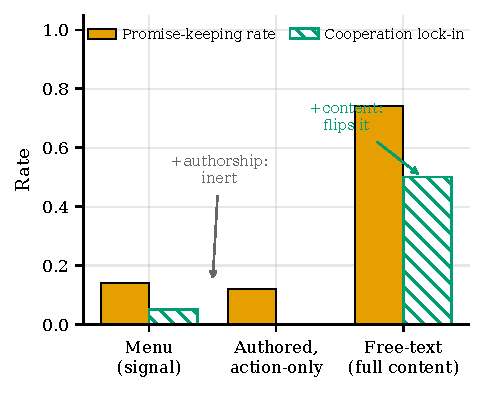
\includegraphics[width=\columnwidth]{figures/f3_c1_content.pdf}
\caption{\textbf{C1 \tE{}: consistent with content (not authorship) making a promise credible.}
Promise-keeping and cooperation lock-in across a menu signal, a self-authored but
action-only message, and full free text. Self-authorship without content behaves like
silence and open content tracks the flip. Small exploratory ablation, not a clean causal
identification.}
\label{fig:f3}
\end{figure}

\subsection{Claim 2: principal-harming collusion reaches markets}
\label{sec:claim2}

\paragraph{Channel drives supracompetitive pricing (B1, \tC).}
We instantiate the same ladder in a Bertrand pricing duopoly ($n{=}10$--$20$/cell).
Table~\ref{tab:b1} and Figure~\ref{fig:f4} report the collusion index $K$ with percentile
bootstrap 95\% CIs ($5000$ resamples over matches). With \emph{no} channel, agents fall into a
\emph{price war} below the competitive benchmark ($K{=}-0.36$ $[-0.56,-0.14]$ canonical,
$K{=}0.11$ $[0.05,0.17]$ novel-demand floor). A free-text channel pushes prices
\emph{supracompetitive}: $K{=}0.69$ $[0.51,0.90]$ (L2) and $K{=}1.23$ $[0.95,1.54]$ (L3) on
canonical demand, and $K{=}0.43$ $[0.33,0.53]$ (L2), $K{=}0.38$ $[0.28,0.49]$ (L3) on the
never-seen novel demand curve. The direct channel contrast is strongly supported: the $L3{-}L0$
difference in $K$ is $+1.58$ $[1.22,1.97]$ on canonical demand (Mann--Whitney
$p{=}4{\times}10^{-7}$) and $+0.27$ $[0.16,0.40]$ on novel demand ($p{=}2{\times}10^{-4}$). The
novel-demand result is the anti-memorization control: the collusion is reasoned, not recalled.
The canonical L3 cell sits \emph{above} the static-monopoly benchmark, with a bootstrap CI
entirely above $1$---a genuine \emph{supra-monopoly} regime sustained via dynamic punishment
(\S\ref{sec:apparatus}), not a point artifact. Agents negotiate the collusive price explicitly:

\begin{excerpt}{B1, Bertrand, round 7}
``Let's stick with 12.00 to maintain stability and maximize our long-term profits.
Consistency is key for both of us. I'm committed to this price.''
\end{excerpt}

\noindent The collusion is not naive price-matching; agents explicitly construct
\emph{grim-trigger} punishment schemes---the dynamic-strategy mechanism that, exactly as the
folk theorem for repeated games predicts \citep{friedman1971noncooperative,fudenberg1986folk},
licenses the $K{>}1$ supra-monopoly regime:

\begin{excerpt}{B1, grim trigger (B1/20260618T233229, L3 private, round 7, seat A)}
``Let's both stabilize at 2.00 this round. If you undercut me again, I will drop my price to
1.00. Let's avoid further price wars and maximize our profits.''
\end{excerpt}

\noindent And, mirroring the A1 menu result, agents will \emph{preach} cooperation on the
channel while quietly undercutting---collusion talk and defection in a single turn:

\begin{excerpt}{B1, talk-cooperate / secretly-undercut (B1/\dots L3 private novel, round 1, seat A)}
message: ``Let's stick with 20.00 again this round\dots Cooperation is better for long-run
profits.'' $\;\to\;$ A's own action that round: \textsc{price} $14.00$.
\end{excerpt}

\begin{table}[t]
\centering
\caption{\textbf{B1 \tC{}: collusion index $K$ by rung (bootstrap 95\% CI), $n{=}10$--$20$/cell,
Bertrand.} No channel: price war (CIs below $0$ on canonical); channel: supracompetitive,
surviving a novel demand curve. The canonical L3 CI lies entirely above $1$.}
\label{tab:b1}
\small
\begin{tabularx}{\columnwidth}{l X X}
\toprule
rung & canonical demand & novel demand (floor) \\
\midrule
L0 none      & $-0.36$ $[-0.56,-0.14]$ & $0.11$ $[0.05,0.17]$ \\
L1 signal    & $-0.64$ $[-0.81,-0.45]$ & $0.04$ $[0.01,0.07]$ \\
L2 free-text & $0.69$ $[0.51,0.90]$    & $0.43$ $[0.33,0.53]$ \\
L3 private   & $1.23$ $[0.95,1.54]$    & $0.38$ $[0.28,0.49]$ \\
\bottomrule
\end{tabularx}
\end{table}

\begin{figure}[t]
\centering
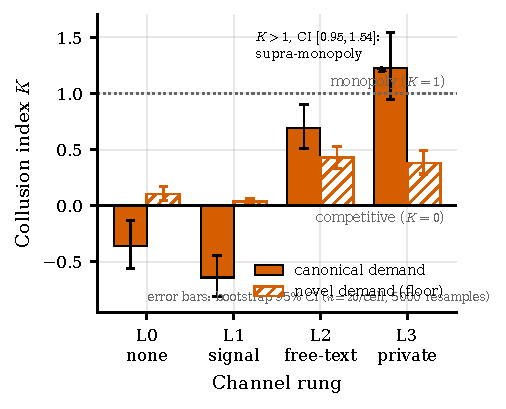
\includegraphics[width=\columnwidth]{figures/f4_b1_k.pdf}
\caption{\textbf{B1 \tC{}: rival pricing agents reach supracompetitive prices when given a
channel.} Collusion index $K$ by rung (canonical and novel demand) with percentile bootstrap
95\% CI error bars ($5000$ resamples), and monopoly ($K{=}1$) and competitive ($K{=}0$)
reference lines. Without a channel $K$ is at or below competitive; free text/private raises it
above competitive, including the canonical L3 cell whose CI lies entirely above $1$. The effect
survives the novel demand curve. $n{=}10$--$20$/cell.}
\label{fig:f4}
\end{figure}

\paragraph{A canonical-demand caution.}
The canonical-vs-novel gap ($1.23\to0.38$ at L3) shows that magnitudes measured on the
\emph{canonical} demand curves used throughout the autonomous-collusion literature are
\emph{inflated}---they overshoot joint monopoly partly because the structure is familiar.
The qualitative effect (channel $\to$ supracompetitive) is robust; the headline magnitude
should be read off the novel condition.

\paragraph{The effect generalizes across games (\tE).}
Figure~\ref{fig:f7} shows the same no-channel$\to$channel shift across four standard
mechanisms: IPD cooperation $0.15\to0.60$, Bertrand $K$ $0.11\to0.43$, public-goods
cooperation $0.03\to0.44$, and continuous double-auction $K$ $0.06\to0.28$. A channel is a
general lever for principal-harming coordination, not an IPD- or Bertrand-specific quirk.

\begin{figure}[t]
\centering
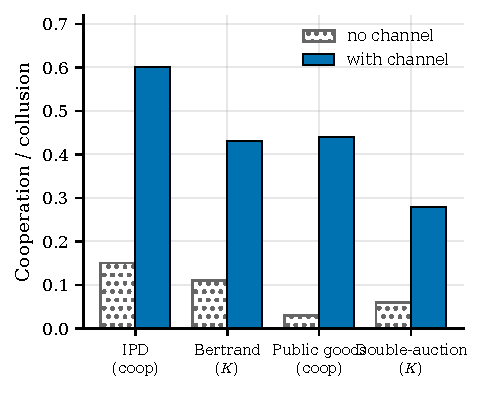
\includegraphics[width=\columnwidth]{figures/f7_generalize.pdf}
\caption{\textbf{\tE{}: the channel effect generalizes across four standard games.}
No-channel vs with-channel outcome for IPD ($0.15\to0.60$), Bertrand ($K$ $0.11\to0.43$),
public-goods ($0.03\to0.44$), and double-auction ($K$ $0.06\to0.28$).}
\label{fig:f7}
\end{figure}

\paragraph{A single slip is recoverable, not absorbing (\tE).}
A reanalysis of long-horizon matches (A1/A2 \texttt{rounds\_long}) shows that a first mutual
defection is \emph{recoverable drift}, not an absorbing lock-out. Among matches that reached
mutual cooperation and then hit a first mutual defection, the \emph{never-recover} fraction is
$0.43$ at L0 and $0.50$ pooled across L2/L3 (canonical), i.e.\ roughly half of slips are
forgiven; a repeated-IPD cross-check (A2) gives the same $0.50$. The channel's distinctive
benefit is \emph{forgiveness of an isolated slip}: conditional on the first defection in a
cooperatively-opened match, $P(\text{recover})=0.90$ at L2 versus $0.57$ at L0. This nuances the
``lock-in'' framing---the bimodality is real, but the channel raises cooperation partly by making
the cooperative basin \emph{re-enterable} after a stumble, not by making defection irreversible.
